\chapter{Algorytm transformacji falkowej}

Algorytm transformacji falkowej, oznaczany skrótem \enquote{WT} (ang. \enquote{Wavelet Transform}), jest przekształceniem umożliwiającym analizę przetwarzanego sygnału w dziedzinie skala-czas~\cite{wallen_handbook}. Skala w przypadku algorytmu transformacji falkowej stanowi wybrany zakres częstotliwości składowych (harmonicznych) analizowanego sygnału. Jest to podobna cecha, jak w przypadku algorytmu \enquote{STFT} (ang. \enquote{Short-Time Fourier Transform})~\cite{durak_sftp}, będącego modyfikacją transformacji Fouriera. W ogólnej formie algorytm ciągłej transformacji falkowej (\enquote{CWT} -- ang. \enquote{Continous Wavelet Transform}) opisać można równaniem~\cite{lord_guide, wallen_handbook}:
\begin{equation}
w_{a,b} = \frac{1}{\sqrt{a}} \int _{-\infty} ^{\infty} x \emb{t} \psi \emb{\frac{t-b}{a}} dt \label{eq:cwt},
\end{equation}
gdzie $w$ jest wyznaczonym współczynnikiem transformacji falkowej, $a$ parametrem skali, $b$ parametrem przesunięcia w czasie, natomiast $\psi(t)$ równaniem falki-matki.

Parametr skali określa zakres częstotliwości -- im większa wartość tego parametru, tym falka staje się bardziej \enquote{rozciągnięta}, przez co odpowiada niższym częstotliwością sygnału ($a > 1$); w przypadku niskich wartości parametru skali ($a < 1$) falka staje się co raz bardziej \enquote{zwarta}, co odpowiada wyższym zakresom częstotliwości. Parametr przesunięcia w czasie określa okno pomiarowe dla wybranego współczynnika. Wybór równania falki-matki zależy od charakteru przetwarzanego sygnału oraz pożądanych właściwości falki. Literatura opisuje bardzo wiele różnych rodzajów falek, wraz z odpowiednimi dla nich obszarami zastosowań~\cite{wallen_handbook, akujuobi_applications}.

Główny podział falek pod katem ich właściwości obejmuje obecność najważniejszych cech charakterystycznych dla danej rodziny: ortogonalność, symetrię oraz biortogonalność. Ortogonalność oznacza, że dla wybranych parametrów skali i przesunięcia w czasie kolejne falki powstałe na bazie falki-matki będą wobec siebie ortogonalne. Jest to cecha w większości przypadków wymagana i pożądana. Symetria funkcji falki-matki jest cenną cechą w przypadku przetwarzania wybranych sygnałów, np. obrazów i dźwięku -- nie wszystkie rodziny falek posiadają tą cechę, stąd wiele prac skupiało się na \enquote{udoskonalaniu} istniejących rodzin pod katem możliwości jej wprowadzenia~\cite{reddy_compression}. Biortogonalność oznacza, że w celu rekonstrukcji sygnału należy zastosować odpowiednią dla użytej falki-matki, powiązaną z nią falkę~\cite{sweldens_bior}.

Ze względu na swoje właściwości, algorytmy transformacji falkowej są wykorzystywane w wielu dziedzinach~\cite{akujuobi_applications}, przy czym w zależności od właściwości analizowanego sygnału stosuje się odpowiednią w danym przypadku falkę-matkę. W medycynie transformacja falkowa wykorzystywana jest między innymi do analizy sygnału EEG oraz EKG~\cite{ocak_medicine, unser_medicine}. Algorytm transformacji falkowej znajduje również zastosowanie w przetwarzaniu obrazu oraz dźwięku~\cite{kotteri_imagecomp}, ze względu na możliwość zastosowania go w algorytmach kompresji danych~\cite{reddy_compression}. Zapewniając możliwości analizy sygnału zarówno w dziedzinie częstotliwości, jak i czasu, algorytmy transformacji falkowej stosowane są w analizie drgań sejsmicznych~\cite{anping_seismic}. Analiza falkowa wykorzystywana jest również w mechanice, gdzie istnieje możliwość oszacowania stanu zużycia elementów mechanicznych maszyn na podstawie wielkości wyjściowych algorytmu transformacji falkowej~\cite{yan_mechanics}, czy w elektroenergetyce w celu analizy zwarć wysokoprądowych~\cite{niedopytalski_zwar}. Jednym z istotnych zastosowań jest także redukcja szumu w sygnale pomiarowym~\cite{auth_denoise}, gdzie wykorzystywane są w dużej mierze falki podwójnej gęstości \enquote{dden}~\cite{vimala_ddendenoise}. Ze względu na fakt, że algorytmy te stanowią istotną część toru pomiarowego, ich właściwości metrologiczne nie mogą być pomijane podczas analizy właściwości metrologicznych tego obiektu.

\section{Algorytm ciągłej transformacji falkowej}

Algorytm ciągłej transformacji falkowej może być stosowany między innymi w celu detekcji, czy oraz w jakim czasie widmo analizowanego sygnału zawierało wybrane harmoniczne~\cite{anping_seismic}. W tym przypadku istnieje możliwość wyznaczenia dowolnej liczby współczynników transformacji, gdzie ich liczba zależy od wymaganej rozdzielczości w skali czasu i częstotliwości~\cite{wallen_handbook}. W przypadku tej wersji algorytmu rozdzielczość w dziedzinie czasu jest zwykle stała i nie zmienia się dla kolejnych skal częstotliwości. Na podstawie widma sygnału można określić w jakim czasie miało miejsce badane zjawisko, wiedząc jaka częstotliwość sygnału jest związana z tym zjawiskiem.

Algorytm ciągłej transformacji falkowej wymaga zastosowania opisanej ciągłym w dziedzinie czasu oraz częstotliwości równaniem falki-matki, natomiast nie wymaga aby określona była funkcja skalująca, której rola i znaczenie zostały opisane w dalszej części pracy. Falki stosowane w przypadku algorytmu ciągłej transformacji falkowej mogą być opisane zarówno w dziedzinie liczb rzeczywistych, jak i zespolonych. Ze względu na możliwość stosowania dowolnych wartości parametru skali i czasu, kolejne falki na bazie falki-matki nie są wobec siebie ortogonalne, co w praktyce oznacza że wyznaczane są w tym przypadku nadmiarowe współczynniki transformacji. Jako, że wyznaczenie nieskończonej liczby współczynników transformacji nie jest możliwe, a dodatkowo z punktu widzenia analizy i przetwarzania sygnałów wyznaczanie nadmiarowych współczynników transformacji nie jest potrzebne, praca nie została poświęcona algorytmom ciągłej transformacji falkowej. W praktyce pomiarowej najczęściej wykorzystuje się algorytmy dyskretnej transformacji falkowej~\cite{wallen_handbook, akujuobi_applications}.

\section{Algorytm dyskretnej transformacji falkowej}

Jak wcześniej wspomniano, wyznaczenie nieskończonej liczby współczynników algorytmu ciągłej transformacji falkowej jest niemożliwe. Wprowadzając ograniczenie możliwych wartości parametrów skali i czasu użytych w równaniu~\eqref{eq:cwt}, w którym $a = 2^m$, $b = n2^m$ oraz $m, n \in \mathbb{N}$, uzyskuje się zależność opisującą algorytm dyskretnej transformacji falkowej (\enquote{DWT} -- ang. \enquote{Discrete Wavelet Transform})~\cite{wallen_handbook}, gdzie $m$ jest numerem skali, a $n$ numerem przesunięcia w czasie (numerem okna pomiarowego). Termin \enquote{dyskretna} oznacza zatem ograniczony (dyskretny) zbiór możliwych wartości dla parametrów skali i przesunięcia w czasie.

Modyfikacja fragmentu równania~\eqref{eq:cwt} wprowadzająca opisywane założenie dyskretyzacji parametrów skali oraz czasu, a następnie założenie początkowych wartości parametrów skali i czasu, gdzie $a_{0} = 2$ oraz $b_{0} = 1$, pozwalają uzyskać zależność opisującą kolejne falki stworzone na bazie falki-matki dla dyskretnych wartości parametru numeru skali $m$ i przesunięcia w czasie $n$:
\begin{equation}
\psi_{m,n} \emb{t} = \psi \emb{\frac{t - n 2^{m}}{2^{m}}} \label{eq:dwt_wavelet}.
\end{equation}
Tak opisana falka jest zwykle ortogonalna oraz musi posiadać znormalizowaną energię, przy czym właściwości te można opisać w postaci:
\begin{equation}
\int _{-\infty} ^{\infty} \psi_{m,n} \emb{t} \psi_{m',n'} \emb{t} dt =
\begin{cases}
	1 & $dla $ m = m' $ oraz $ n = n' \\
	0 & $w pozostałych przypadkach$
\end{cases}
\label{eq:dwt_orthogonal_mather}.
\end{equation}
W praktyce oznacza to, że nie ma możliwości opisu dowolnej, stworzonej na podstawie równania~\eqref{eq:dwt} falki pochodnej, za pomocą bazującej na tej samej falce-matce falki o innym numerze skali lub czasu.

Podstawiając falkę opisaną równaniem~\eqref{eq:dwt_wavelet} do równania~\eqref{eq:cwt} dla przyjętych założeń otrzymuje się zależność opisującą dyskretną transformację falkową~\cite{shensa_dwt}:
\begin{equation}
w_{m,n} = \frac{1}{\sqrt{2^{m}}} \int _{-\infty} ^{\infty} x \emb{t} \psi \emb{\frac{t - n 2^{m}}{2^{m}}} dt \label{eq:dwt}.
\end{equation}
Cechą algorytmu dyskretnej transformacji falkowej jest dynamiczna zależność rozdzielczości dziedziny czasu w funkcji skali. Dla niskich wartości parametru skali, które odpowiadać będą wysokim częstotliwościom przetwarzanego sygnału, rozdzielczość w dziedzinie czasu jest większa w porównaniu z rozdzielczością dla skali wyższych, które odpowiadać będą niższym zakresom częstotliwości przetwarzanego sygnału. Jako, że sygnał o wyższej częstotliwości zmienia się bardziej dynamicznie, niż ma to miejsce w przypadku sygnału o niższej częstotliwości, takie podejście jest bardzo korzystne. Umożliwia ono redukcję liczby współczynników transformacji, a zatem redukcję liczby wielkości wyjściowych analizowanego algorytmu, przy jednoczesnym zachowaniu optymalnej rozdzielczości w dziedzinie czasu oraz zapewnieniu możliwości rekonstrukcji oryginalnego przebiegu sygnału na podstawie uzyskanych współczynników transformacji.

Mając na uwadze fakt, że falka-matka dla wybranego numeru skali stanowi filtr pasmowo-przepustowy, przy czym zwiększanie tego numeru powoduje przesunięcie charakterystyki filtru w kierunku niższych częstotliwości, w celu wyodrębnienia wszystkich częstotliwości z przetwarzanego sygnału należy wyznaczyć wartości współczynników transformacji dla nieskończonej liczby skal -- w innym wypadku wszystkie niskie zakresy częstotliwości nie zostaną przetworzone. Naturalnie, nie jest to w praktyce możliwe. Aby rozwiązać problem analizy niskich częstotliwości przetwarzanego sygnału, stosuje się tzw. \enquote{funkcję skalującą} nazywaną również \enquote{falką-ojcem}~\cite{shensa_dwt}. Funkcja ta, w przeciwieństwie do falki-matki, stanowi filtr dolno-przepustowy i zastępuje określony przedział niskich skal falki-matki -- w ten sposób eliminuje się potrzebę wyznaczania nieskończonej liczby współczynników transformacji przy jednoczesnej możliwości analizy całego widma przetwarzanego sygnału. Funkcja skalująca jest ściśle powiązana z falką-matką i jest oznaczana w literaturze jako $\phi(t)$~\cite{wallen_handbook}. Można w tym miejscu zauważyć, że aby dana rodzina falek mogła zostać wykorzystana przez algorytm dyskretnej transformacji falkowej, musi być dla niej określona odpowiednia funkcja skalująca.

Stosując założenia ograniczenia zbioru wartości parametrów skali i przesunięcia w czasie, zależność opisującą funkcję skalującą przedstawić można w postaci~\cite{ahmad_wavelet}:
\begin{equation}
\phi_{m,n} \emb{t} = \frac{1}{\sqrt{2^{m}}} \phi \emb{\frac{t - n 2^{m}}{2^{m}}} \label{eq:dwt_scalefun},
\end{equation}
przy czym funkcję tą dla $m = n = 0$ nazywa się w literaturze \enquote{falką-ojcem}~\cite{akujuobi_applications}. Właściwością funkcji skalującej jest spełnianie przez nią założenia odnośnie ograniczonej energii oraz ortogonalność względem samej siebie dla dowolnych różnych wartości parametru numeru przesunięcia w czasie~\cite{ahmad_wavelet}:
\begin{equation}
\int _{-\infty} ^{\infty} \phi_{m,n} \emb{t} \phi_{m',n'} \emb{t} dt =
\begin{cases}
	0 & $dla $ n \ne n' \\
	1 & $w pozostałych przypadkach$
\end{cases}
\label{eq:dwt_orthogonal_father}.
\end{equation}
Warto zaznaczyć, że w przypadku zmiany parametru numeru skali kolejne wersje funkcji skalującej nie są wobec siebie ortogonalne. W praktyce jednak nie ma to znaczenia, ponieważ współczynniki transformacji zależne od funkcji skalującej wyznacza się tylko dla jednej wartości parametru numeru skali oraz dla wszystkich dostępnych wartości parametru numeru przesunięcia w czasie.

Omawianą funkcję skalującą można przedstawić również w postaci sumy iloczynów współczynników skalowania oraz wartości przeskalowanej i przesuniętej w czasie funkcji skalującej, co opisuje następującą zależność~\cite{wallen_handbook}:
\begin{equation}
\phi \emb{t} = \sum _{k=0} ^{N_k-1} c_{k} \phi \left( 2t - k \right) \label{eq:dwt_scalefunrek},
\end{equation}
gdzie $k$ jest dowolną liczbą całkowitą powiązaną ze współczynnikiem skalowania $c_k$. Kolejne wartości współczynników $c_k$ muszą dodatkowo spełniać warunek~\cite{wallen_handbook}:
\begin{equation}
\sum _{k=0} ^{N_k-1} c_{k} = 2 \label{eq:dwt_scalefunsum}.
\end{equation}
Należy również zaznaczyć, że w celu zachowania warunku wzajemnej ortogonalności opisywanej rodziny falek, spełnione musi zostać dodatkowe założenie odnośnie wzajemnej relacji pomiędzy kolejnymi wartościami współczynników skalowania, w którym przyjmuje się że~\cite{akujuobi_applications}:
\begin{equation}
\sum _{k=0} ^{N_k-1} c_{k} c_{k+2k'} =
\begin{cases}
	2 & $gdy$~k' = 0 \\
	0 & $w pozostałych przypadkach$
\end{cases}
\label{eq:dwt_scalemulort}.
\end{equation}
Powyższe założenia zapewniają ortogonalność stworzonych falek w stosunku do funkcji skalującej oraz brak nadmiarowych wielkości wyjściowych algorytmu dyskretnej transformacji falkowej. Tworzone na opisanych zasadach falki posiadają skończoną liczbę niezerowych współczynników skalujących $c_k$, przy czym rząd falki $N_r$ określa liczbę tych współczynników równą $N_{k} = 2 N_r$~\cite{lord_guide}. Manipulując znakiem i kolejnością współczynników skalujących istnieje możliwość opisu falki-matki w postaci~\cite{wallen_handbook}:
\begin{equation}
\psi \emb{t} = \sum _{k=0} ^{N_k-1} \emb{-1} ^{k} c_{N_k-k-1} \phi \left( 2t - k \right) \label{eq:dwt_waveletfunrek}.
\end{equation}
Ostatecznie przedstawić można rekursywne zależności opisujące funkcję skalującą i funkcję falki dla dowolnego numeru skali i numeru przesunięcia czasowego za pomocą równań:
\begin{gather}
\psi_{m+1,n} \emb{t} = \frac{1}{\sqrt{2}} \sum _{k=0} ^{N_k-1} c_{k} \psi_{m,2n+k} \emb{t} \label{eq:dwt_fatherrek}, \\
\phi_{m+1,n} \emb{t} = \frac{1}{\sqrt{2}} \sum _{k=0} ^{N_k-1} b_{k} \psi_{m,2n+k} \emb{t} \label{eq:dwt_matherrek},
\end{gather}
przy czym parametr $b_{k}$ przedstawić można jako rekombinacje współczynników skalujących $c_{k}$ określoną równaniem:
\begin{equation}
b_{k} = \emb{-1} ^{k} c_{N_k-k-1} \label{eq:dwt_bk}.
\end{equation}

Dekompozycja przetwarzanego sygnału w przypadku algorytmu dyskretnej transformacji falkowej odbywa się w ten sposób, że sygnał wejściowy podawany jest na wejścia pary filtrów -- górno i dolno przepustowego. Wyjście filtru dolno przepustowego stanowi aproksymacje sygnału, natomiast wyjście filtru górno przepustowego stanowią detale sygnału. Ze względu na fakt, że opisywana operacja dostarcza dwa razy więcej próbek wyjściowych, niż zawierał oryginalny sygnał, co druga próbka wyjściowa jest usuwana w procesie decymacji~\cite{lord_guide}. Opisywane działanie rozdziela widmo sygnału na dwie części: detale sygnału związane z wysokimi częstotliwościami oraz aproksymacje sygnału powiązaną z niskimi zakresami częstotliwości składowych tego sygnału. Filtr dolno-przepustowy odpowiada charakterystyce funkcji skalującej, natomiast filtr górno-przepustowy charakterystyce falki-matki. Filtr górno-przepustowy jest więc faktycznie filtrem pasmowo-rzepustowym, natomiast ze względu na wartość parametru skali jego częstotliwość środkowa odpowiada częstotliwości Nyquista dla przetwarzanego sygnału -- stąd też można nazwać go filtrem górno-przepustowym~\cite{ahmad_wavelet}. Proces dekompozycji sygnału może zostać powtórzony dla aproksymacji sygnału wielokrotnie, zapewniając większą rozdzielczość w dziedzinie częstotliwości kosztem mniejszej rozdzielczości w dziedzinie czasu~\cite{vonesch_dbbasics}. Przebieg procesu dekompozycji sygnału dla trzech iteracji tego procesu przedstawiono na rysunku~\ref{fig:dwt_decomposition}.

W celu rekonstrukcji sygnału należy zastosować odpowiedni bank filtrów, który w parze z bankiem filtrów wejściowych stanowi system zwany kwadraturowymi filtrami lustrzanymi~\cite{johnston_filter}. Na wejście opisywanego filtru podać należy współczynniki uzyskane wcześniej na drodze dekompozycji sygnału wykonanej za pomocą lustrzanego filtru. Przebieg procesu rekonstrukcji sygnału dla trzech iteracji opisywanego procesu przedstawiono na rysunku~\ref{fig:dwt_reconstruction}.

Na rysunkach~\ref{fig:dwt_decomposition} oraz~\ref{fig:dwt_reconstruction} \enquote{strzałką w górę} oznaczono uzupełnianie brakujących wielkości wejściowych współczynnikami o wartości zero. Działanie to wynika z faktu, że liczba wielkości wejściowych jest mniejsza, niż liczba wielkości wyjściowych. \enquote{Strzałką w dół} oznaczono natomiast proces decymacji, czyli odrzucania co drugiej wielkości wyjściowej. Pominięcie tego procesu spowodowałoby, że wielkości wyjściowych byłoby dwa razy więcej, niż jest to wymagane w celu rekonstrukcji sygnału. Symbol $S$ na rysunkach oznacza wielkości wyjściowe związane z detalami sygnału, a symbol $T$ wielkości wyjściowe związane z aproksymacją sygnału. Indeks dolny związany jest z numerem iteracji procesu dekompozycji. Opisywany algorytm w literaturze nosi nazwę \enquote{Algorytm Malata} lub \enquote{FWT} (ang. \enquote{Fast Wavelet Transform}) i został opracowany w 1988 roku przez Stéphane Mallata~\cite{lujian_mallat}.

\begin{figure}[htb!]
\begin{center}
\includegraphics{obrazki/dwt_dekompozycja}
\makecaption{fig:dwt_decomposition}{Proces dekompozycji sygnału za pomocą algorytmu Mallata}
\end{center}
\end{figure}

\begin{figure}[htb!]
\begin{center}
\includegraphics{obrazki/dwt_rekonstrukcja}
\makecaption{fig:dwt_reconstruction}{Proces rekonstrukcji sygnału za pomocą algorytmu Mallata}
\end{center}
\end{figure}

Pominiecie procesu decymacji powoduje powstanie nadmiarowych wielkości wyjściowych algorytmu i jest praktykowane w przypadku algorytmu \enquote{UWT} (ang. \enquote{Undecimated Wavelet Transform})~\cite{lord_guide}. W omawianym przypadku dla każdego poziomu dekompozycji wyznaczanych jest tyle wielkości wyjściowych, ile wielkości wejściowych zawierał przetwarzany sygnał. Analiza falkowa z pominięciem procesu decymacji znajduje swoje zastosowanie między innymi w przetwarzaniu sygnałów dla celów automatyki elektroenergetycznej~\cite{niedopytalski_ene}, przy czym realizacja procesu dekompozycji przebiega w tym przypadku podobnie, jak w przypadku numerycznej realizacji algorytmu ciągłej transformacji falkowej~\cite{lord_guide}. Innym przypadkiem, w którym liczba wielkości wyjściowych jest większa od liczby wielkości wyjściowych jest przypadek dotyczący rodziny falek podwójnej gęstości, gdzie na każdym etapie dekompozycji stosuje się dodatkową parę filtrów~\cite{selenick_ddenusage}.

Zgodnie z przedstawionymi dotychczas zależnościami, omawiany proces dekompozycji sygnału można opisać również rekurencyjnie za pomocą równań~\cite{wallen_handbook}:
\begin{gather}
S_{m+1,n} = \frac{1}{\sqrt{2}} \sum _{k=0} ^{N_k-1} c_{k} S_{m,2n+k} \label{eq:dwt_aproxrek}, \\
T_{m+1,n} = \frac{1}{\sqrt{2}} \sum _{k=0} ^{N_k-1} b_{k} S_{m,2n+k} \label{eq:dwt_detailrek},
\end{gather}
natomiast proces rekonstrukcji sygnału opisać można rekurencyjne za pomocą równania:
\begin{equation}
S_{m-1,n} = \frac{1}{\sqrt{2}} \left( \sum _{k=0} ^{N_k-1} c_{n-2k} S_{m,k} + \sum _{k=0} ^{N_k-1} b_{n-2k} T_{m,k} \right) \label{eq:dwt_reconrek},
\end{equation}
gdzie $S_{0,i}$ jest $i$-tą próbką przetwarzanego sygnału, $S_{m+1,n}$ aproksymacjami oraz $T_{m+1,n}$ detalami sygnału dla zadanego numeru skali $m$ i przesunięcia w czasie $n$. Współczynniki $c_i$ oraz $b_i$ są niezerowe tylko dla $i$ należących do przedziału $<0;N_k-1>$ -- poza tym przedziałem są one równe zero. Wartości i liczba współczynników $c$ oraz $b$ zależą od zastosowanej rodziny falek i jej rzędu. W przypadku, gdy w wektorze wielkości wejściowych nie istnieje element o zadanym indeksie (tj. zachodzi $S_{m,i}$ lub $T_{m,i}$ dla $i \ge N$) należy przyjąć w obliczeniach wartość dla indeksu $i' = i \text{ mod } N$, gdzie \enquote{mod} jest resztą z dzielenia wyrazu po lewej stronie operatora przez wyraz z prawej strony operatora. Identycznie postępować należy w przypadku procesu rekonstrukcji sygnału.

Ze względu na fakt, że ciągła transformacja falkowa jest w praktyce niemożliwa w realizacji, natomiast proces decymacji nie jest zwykle pomijany ze względu na brak potrzeby wyznaczania nadmiarowej liczby współczynników, dalsza część pracy poświęcona będzie algorytmowi dyskretnej transformacji falkowej. Przedstawiany w pracy sposób analizy właściwości metrologicznych będzie jednak jednolity dla rzeczywistych implementacji omawianych algorytmów.

\section{Bank filtrów algorytmu}

Zależnie od wymaganych kryteriów podczas stosowania algorytmów transformacji falkowej wybiera się odpowiednią do analizowanego sygnału falkę-matkę. Wybór falki-matki ma ogromny wpływ na proces dekompozycji sygnału, ponieważ to właśnie od niej zależą parametry banku filtrów, na którego wejście podawany jest przetwarzany przez algorytm sygnał. W przypadku algorytmów ciągłej transformacji falkowej istnieje możliwość zastosowania dowolnie dużej liczby kombinacji wartości parametru skali i przesunięcia w czasie, przez co dekompozycja sygnału jest bardziej dokładna.

Na rysunkach~\ref{fig:demo_db} oraz~\ref{fig:demo_spline} zaprezentowano przykładowe banki filtrów, gdzie na osi poziomej przedstawiono częstotliwość znormalizowaną do połowy częstotliwości próbkowania (częstotliwości Nyquista), a na osi pionowej znormalizowane do jedności wzmocnienie. Wzmocnienie zostało znormalizowane z osobna dla każdego poziomu dekompozycji w celu uczytelnienia wykresów i możliwości ich łatwiejszego porównywania. Kolorem niebieskim oznaczono na rysunkach charakterystyki filtru dolno-przepustowego powstałego na bazie funkcji skalującej. Pozostałe filtry powstały na bazie odpowiednio przeskalowanej falki-matki. Należy zauważyć, że w przypadku dyskretnej wersji algorytmu transformacji falkowej, w praktyce liczba etapów procesu dekompozycji jest ograniczona -- wraz ze zwiększaniem tej liczby maleje rozdzielczość w skali czasu dla aproksymacji sygnału, aż do chwili gdy aproksymacje sygnału stanowi jedna wielkość wyjściowa~\cite{wallen_handbook}.

\begin{figure}[htb!]
\begin{center}
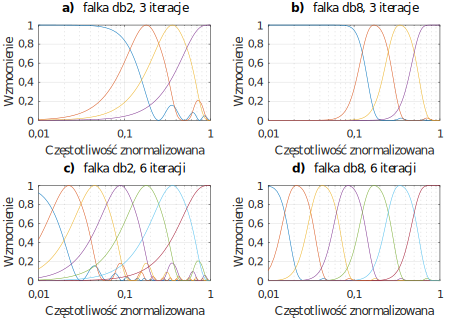
\includegraphics{obrazki/bank_db_demo}
\makecaption{fig:demo_db}{Przykładowe banki filtrów dla rodziny falek \enquote{Daubechies}}
\end{center}
\end{figure}

Na podstawie wykresu zauważyć można, że dla kolejnych parametrów skali pasmo przenoszenia filtru jest o połowę mniejsze w stosunku do pasma przenoszenia filtru poprzedniej skali. Zgodnie z przedstawionymi charakterystykami, kolejne etapy dekompozycji sygnału przenoszą zatem fragment widma analizowanego sygnału zgodnie z charakterystyką zastosowanej falki-matki. Zależnie od właściwości falki-matki zbudowane na jej podstawie filtry mogą być mniej lub bardziej selektywne (wykazywać inną stromość charakterystyki filtru), czy też wykazywać cechy filtrów grzebieniowych (mogą przenosić kilka zakresów częstotliwości). Im bardziej skomplikowany będzie kształt falki i wyższy będzie jej rząd, tym zwykle bardziej selektywny będzie filtr stworzony na jej bazie. Wzrost liczby iteracji dekompozycji sygnału wprowadza kolejne filtry o węższym niż dla mniejszej liczby iteracji paśmie przenoszenia. Z analizy przedstawionych rysunków wynika, że w przypadku wszystkich przedstawionych rodzin falek, wzrost rzędu falki powoduje wzrost selektywności kolejnych filtrów. Część z przedstawionych falek zapewnia filtry podobne do filtrów grzebieniowych -- pasmo przenoszenia tych filtrów składa się z kilku przedziałów częstotliwości.

\begin{figure}[htb!]
\begin{center}
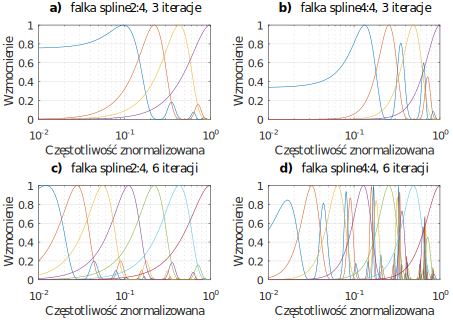
\includegraphics{obrazki/bank_spline_demo}
\makecaption{fig:demo_spline}{Przykładowe banki filtrów dla rodziny falek \enquote{Spline}}
\end{center}
\end{figure}

Przedstawiona na osi pionowej maksymalna wartość wzmocnienia w funkcji częstotliwości sygnału może być w rzeczywistości większa od jedności. W praktyce każdy z fragmentów banku filtrów traktować można jako pasmowo-przepustowy filtr cyfrowy i opisywać za pomocą modelu filtru o skończonej odpowiedzi impulsowej (\enquote{FIR}). Z punktu widzenia pojedynczej wielkości wyjściowej, algorytm transformacji falkowej może być zatem rozumiany jako odpowiednio zaprojektowany filtr, który z sygnału wejściowego przenosi na wyjście wybrane harmoniczne sygnału wejściowego z odpowiednim wzmocnieniem i przesunięciem fazowym. Przedstawione cechy banku filtrów będą bardzo istotne w dalszym etapie pracy w szczególności do określania, w jaki sposób algorytm przenosi błędy opisane w pracy jako dynamiczne. Należy zauważyć, że skoro kolejne filtry w banku odpowiadają kolejnym etapom dekompozycji sygnału, to w większości przypadków właściwości metrologiczne będą jednakowe dla wszystkich wielkości wyjściowych powiązanych z identycznym etapem dekompozycji sygnału, co znacznie upraszcza proces analizy właściwości metrologicznych omawianych algorytmów. W pewnych przypadkach jednak wypadkowe właściwości toru pomiarowego mogą ulec zmianie, jeżeli wprowadzona zostanie dodatkowa modyfikacja wielkości wejściowych algorytmu transformacji falkowej (np. wprowadzone zostanie okno pomiarowe). Należy w takim przypadku analizować właściwości metrologiczne każdej wielkości wyjściowej z osobna, a nie, jak w klasycznym przypadku, analizować je zbiorczo dla danego etapu dekompozycji

\section{Macierzowa postać algorytmu}

Ze względu na bardzo dużą liczbę opisanych w literaturze falek~\cite{akujuobi_applications}, ich unikatowe właściwości oraz możliwość zmiany parametrów procesu dekompozycji sygnału, metody analityczne określenia właściwości metrologicznych dla wybranej kombinacji parametrów okazują się czasochłonne i niepraktyczne~\cite{yan_uncertainty, wilczok_uncertainty, peretto_uncertainty, sarrafi_uncertainty}. Część opisywanych w literaturze falek obejmuje falki: \enquote{Daubechies}~\cite{vonesch_dbbasics}, \enquote{Haara}~\cite{stankovic_haar}, \enquote{Coiflet}~\cite{wei_coiflet}, \enquote{Biortogonalne}~\cite{sweldens_bior}, \enquote{Morleta}~\cite{cohen_morlet}, \enquote{Meksykańskiej czapki}~\cite{singh_mexican}, \enquote{Spline}~\cite{averbuch_spline, wang_splinebasics}. Każdą falkę oraz przypisaną do niej funkcję skalującą opisują odpowiednie równania, przy czym nie zawsze są one zadane w postaci jawnej -- w wielu przypadkach rodzina falek opisana jest przez zbiór zależności określających wymagane przez nią założenia, co jeszcze bardziej komplikuje proces analizy tych algorytmów~\cite{rowe_dbmath}. Podczas projektowania toru pomiarowego często istnieje potrzeba zmiany parametrów algorytmu transformacji falkowej, co pociąga za sobą konieczność przeprowadzenia powtórnej analizy jego właściwości metrologicznych. Wszystkie te czynniki sprawiają, że analiza ta jest najczęściej pomijana w pracach opisujących aplikacje omawianych algorytmów. Z opisywanych właściwości algorytmów transformacji falkowej wynika potrzeba przedstawienia uniwersalnej metody umożliwiającej analizę właściwości metrologicznych tych algorytmów. Metoda ta musi być przystępna w aplikacji oraz musi zakładać, że projektant toru pomiarowego nie jest ekspertem w dziedzinie transformacji falkowej, a jedynie użytkownikiem tej transformacji. Co więcej, ewentualna zmiana parametrów zastosowanego algorytmu nie może być kłopotliwa z punktu widzenia określenia nowych właściwości metrologicznych analizowanego algorytmu.

Problem skomplikowanej analizy algorytmów transformacji falkowej, podobnie jak w przypadku innych algorytmów przetwarzających ciągi danych, uprościć można przedstawiając analizowany algorytm w postaci macierzowej. Wektor wielkości wyjściowych algorytmu jest wtedy równy iloczynowi macierzy transformacji i wektora wielkości wejściowych zgodnie z równaniem~\eqref{eq:alg_out_mat}. Przedstawienie algorytmu transformacji falkowej w formie macierzowej umożliwi stworzenie jednolitego i uniwersalnego opisu działania tego algorytmu oraz w znaczącym stopniu ułatwi jego analizę w kolejnych rozdziałach pracy. Zwykle projektant toru pomiarowego nie jest ekspertem w dziedzinie falek -- jest on ekspertem w dziedzinie analizowanego zjawiska, a transformacja falkowa jest dla niego jedynie narzędziem, umożliwiającym jego analizę. Stąd, w większości przypadków, osoba ta stosuje gotowe biblioteki zaimplementowane np. dla środowisk \enquote{Matlab}, \enquote{GNU Octave} czy \enquote{PyWavelets}~\cite{lee_pywavelets, misiti_matlabwav}.

W celu identyfikacji wartości współczynników macierzy transformacji należy zastosować metodę opisaną w poprzednim rozdziale pracy lub wyznaczyć te wartości analitycznie, co zostanie przedstawione w dalszej cześć rozdziału. Opisany wcześniej algorytm identyfikacji macierzy transformacji może być zaimplementowany w środowiskach, które implementują algorytmy transformacji falkowej, przez co projektant toru pomiarowego z łatwością jest w stanie go zastosować. Ewentualna zmiana parametrów algorytmu transformacji falkowej (zmiana liczby wielkości wejściowych, liczby iteracji procesu dekompozycji, czy wybór innej falki-matki) skutkować będzie jedynie koniecznością ponownej identyfikacji wartości współczynników macierzy transformacji.

Poza opisanym algorytmem identyfikacji współczynników macierzy transformacji, bazującym na istniejącej implementacji omawianego algorytmu, istnieje możliwość wyznaczenia wartości tych współczynników przy użyciu zależności przedstawionych we wcześniejszej części rozdziału, opisującej właściwości algorytmu dyskretnej transformacji falkowej. Proces ten jest jednak skomplikowany i uzależniony od założeń związanych z opisem zastosowanej falki-matki i jej funkcji skalującej. Poniżej zostanie przedstawiony przykład wyznaczania wartości macierzy transformacji w przypadku zastosowania falki \enquote{db2} dla dwóch iteracji procesu dekompozycji sygnału oraz ośmiu próbek wejściowych sygnału. Macierz transformacji będzie miała zatem wymiary ośmiu wierszy i ośmiu kolumn, natomiast wektor próbek wejściowych oraz wektor próbek wyjściowych będą zawierały po osiem elementów.

Rodzina falek \enquote{Daubechies} (nazywana w skrócie \enquote{db}) została opisana przez Ingrid Daubechies~\cite{vonesch_dbbasics}. Rodzina ta cechuje się ortogonalnością, natomiast nie wykazuje cech symetrii. Poza założeniami opisanymi w poprzednim podrozdziale, danymi w równaniach~\eqref{eq:dwt_orthogonal_mather} oraz od~\eqref{eq:dwt_orthogonal_father} do~\eqref{eq:dwt_scalemulort}, rodzina ta spełnia dodatkowe założenie odnośnie relacji pomiędzy kolejnymi współczynnikami skalującymi, które opisuje następujące równanie~\cite{vonesch_dbbasics}:
\begin{equation}
\sum _{k=0} ^{N_k-1} \emb{-1}^{k} c_{k} k^{m} = 0 \label{eq:db_musthave},
\end{equation}
gdzie $m$ jest liczbą całkowitą z przedziału $<0;\frac{N_{k}}{2}-1>$. W przypadku falek \enquote{db} oraz ich pochodnych, rząd falki wynosi $\frac{N_{k}}{2}$. Falka \enquote{db2}, będąca falką drugiego rzędu, posiada zatem cztery niezerowe współczynniki skalujące. W literaturze spotkać się można również z oznaczeniem \enquote{D4} dla omawianej falki, gdzie zamiast rzędu falki wskazana jest liczba niezerowych współczynników skalujących. Należy zauważyć, że falka \enquote{Daubechies} rzędu pierwszego jest opisana identycznymi zależnościami, jak falka Hara i posiada identyczne właściwości. Z falek \enquote{Daubechies} wywodzą się kolejne rodziny: \enquote{Symleth} oraz \enquote{Coiflet}, które uzupełniają ją o kolejne cechy -- w szczególności symetrię, istotną podczas przetwarzania i analizy obrazów~\cite{wallen_handbook, akujuobi_applications}.

Jako, że falka \enquote{db2} posiada cztery niezerowe współczynniki skalujące oznaczone jako $c_0$, $c_1$, $c_2$, $c_3$, to zgodnie z równaniem~\eqref{eq:dwt_scalefunrek} oraz równaniem~\eqref{eq:dwt_waveletfunrek}, zapisać można równanie falki-matki i funkcji skalującej w postaci:
\begin{gather}
\phi \emb{t} = c_{0} \phi \emb{2t} + c_{1} \phi \left( 2t - 1 \right) + c_{2} \phi \left( 2t - 2 \right) + c_{3} \phi \left( 2t - 3 \right) \label{eq:db2_scalefunrek}, \\
\psi \emb{t} = c_{3} \phi \emb{2t} - c_{2} \phi \left( 2t - 1 \right) + c_{1} \phi \left( 2t - 2 \right) - c_{0} \phi \left( 2t - 3 \right) \label{eq:db2_waveletfunrek}.
\end{gather}
Uwzględniając założenia przedstawione w poprzedniej części rozdziału oraz te wskazane powyżej, zapisać można układ równań wiążący wszystkie przedstawione zależności:
\begin{equation}
\begin{cases}
	c_{0} + c_{1} + c_{2} + c_{3} = 2                 & $na podstawie właściwości~\eqref{eq:dwt_scalefunsum}$ \\
	c_{0}^{2} + c_{1}^{2} + c_{2}^{2} + c_{3}^{2} = 2 & $na podstawie właściwości~\eqref{eq:dwt_scalemulort}$ \\
	c_{0} - c_{1} + c_{2} - c_{3} = 0                 & $na podstawie~\eqref{eq:db_musthave} dla $ m = 0 \\
	- 1 c_{1} + 2 c_{2} - 3 c_{3} = 0                 & $na podstawie~\eqref{eq:db_musthave} dla $ m = 1
\end{cases}
\label{eq:db2_system},
\end{equation}
oraz wskazać jego rozwiązanie, które determinuje następujące wartości kolejnych współczynników skalujących:
\begin{equation}
c_{0} = \frac{1 + \sqrt{3}}{4}, c_{1} = \frac{3 + \sqrt{3}}{4}, c_{2} = \frac{3 - \sqrt{3}}{4}, c_{3} = \frac{1 - \sqrt{3}}{4} \label{eq:db2_coefs},
\end{equation}
przy czym analogicznie postąpić należy w przypadku wyższych rzędów opisywanej falki.

Zgodnie z założeniami odnośnie długości wektora wielkości wejściowych oraz liczby poziomów dekompozycji zauważyć można, że wektor wielkości wyjściowych zawierać będzie dwie próbki związane z aproksymacją sygnału dla skali $m = 2$, dwie próbki związane z detalami sygnału dla skali $m = 2$ oraz cztery próbki związane z detalami dla skali $m = 1$. Oznaczając wektor wielkości wejściowych jako:
\begin{equation}
\mathbf{x}^{T} =
\begin{bmatrix}
S_{0,0} & S_{0,1} & S_{0,2} & S_{0,3} & S_{0,4} & S_{0,5} & S_{0,6} & S_{0,7}
\end{bmatrix}
\label{eq:db2_invect},
\end{equation}
wektor wielkości wyjściowych można opisać w postaci:
\begin{equation}
\mathbf{X}^{T} =
\begin{bmatrix}
S_{2,0} & S_{2,1} & T_{2,0} & T_{2,1} & T_{1,0} & T_{1,1} & T_{1,2} & T_{1,3}
\end{bmatrix}
\label{eq:db2_outvect},
\end{equation}
a następnie zgodnie z równaniem~\eqref{eq:dwt_aproxrek} oraz~\eqref{eq:dwt_detailrek} opisać można kolejne wymienione w równaniu~\eqref{eq:db2_outvect} wielkości wyjściowe za pomocą zależności:
\begin{gather}
S_{2,0} = \frac{1}{\sqrt{2}} \left( c_{0} S_{1,0} + c_{1} S_{1,1} + c_{2} S_{1,2} + c_{3} S_{1,3} \right) \label{eq:db2_outvect_s_2_0}, \\
S_{2,1} = \frac{1}{\sqrt{2}} \left( c_{0} S_{1,2} + c_{1} S_{1,3} + c_{2} S_{1,4} + c_{3} S_{1,5} \right) \label{eq:db2_outvect_s_2_1}, \\
T_{2,0} = \frac{1}{\sqrt{2}} \left( c_{3} S_{1,0} - c_{2} S_{1,1} + c_{1} S_{1,2} - c_{0} S_{1,3} \right) \label{eq:db2_outvect_t_2_0}, \\
T_{2,1} = \frac{1}{\sqrt{2}} \left( c_{3} S_{1,2} - c_{2} S_{1,3} + c_{1} S_{1,4} - c_{0} S_{1,5} \right) \label{eq:db2_outvect_t_2_1}, \\
T_{1,0} = \frac{1}{\sqrt{2}} \left( c_{3} S_{0,0} - c_{2} S_{0,1} + c_{1} S_{0,2} - c_{0} S_{0,3} \right) \label{eq:db2_outvect_t_1_0}, \\
T_{1,1} = \frac{1}{\sqrt{2}} \left( c_{3} S_{0,2} - c_{2} S_{0,3} + c_{1} S_{0,4} - c_{0} S_{0,5} \right) \label{eq:db2_outvect_t_1_1}, \\
T_{1,2} = \frac{1}{\sqrt{2}} \left( c_{3} S_{0,4} - c_{2} S_{0,5} + c_{1} S_{0,6} - c_{0} S_{0,7} \right) \label{eq:db2_outvect_t_1_2}, \\
T_{1,3} = \frac{1}{\sqrt{2}} \left( c_{3} S_{0,6} - c_{2} S_{0,7} + c_{1} S_{0,0} - c_{0} S_{0,1} \right) \label{eq:db2_outvect_t_1_3},
\end{gather}
gdzie $S_{m,n}$ oznaczono aproksymacje, natomiast $T_{m,n}$ detale sygnału dla zadanego numeru skali i numeru przesunięcia w czasie. Po przekształceniu otrzymuje się równania:
\begin{gather}
\begin{split}
S_{2,0} =~
	& \frac{1}{\sqrt{2}} \frac{c_{0}}{\sqrt{2}} \left( c_{0} S_{0,0} + c_{1} S_{0,1} + c_{2} S_{0,2} + c_{3} S_{0,3} \right) + \\
	& \frac{1}{\sqrt{2}} \frac{c_{1}}{\sqrt{2}} \left( c_{0} S_{0,2} + c_{1} S_{0,3} + c_{2} S_{0,4} + c_{3} S_{0,5} \right) + \\
	& \frac{1}{\sqrt{2}} \frac{c_{2}}{\sqrt{2}} \left( c_{0} S_{0,4} + c_{1} S_{0,5} + c_{2} S_{0,6} + c_{3} S_{0,7} \right) + \\
	& \frac{1}{\sqrt{2}} \frac{c_{3}}{\sqrt{2}} \left( c_{0} S_{0,6} + c_{1} S_{0,7} + c_{2} S_{0,0} + c_{3} S_{0,1} \right)
\end{split}
\label{eq:db2_outvect_s_2_0_rek}, \\
\begin{split}
S_{2,1} =~
	& \frac{1}{\sqrt{2}} \frac{c_{0}}{\sqrt{2}} \left( c_{0} S_{0,4} + c_{1} S_{0,5} + c_{2} S_{0,6} + c_{3} S_{0,7} \right) + \\
	& \frac{1}{\sqrt{2}} \frac{c_{1}}{\sqrt{2}} \left( c_{0} S_{0,6} + c_{1} S_{0,7} + c_{2} S_{0,0} + c_{3} S_{0,1} \right) + \\
	& \frac{1}{\sqrt{2}} \frac{c_{2}}{\sqrt{2}} \left( c_{0} S_{0,0} + c_{1} S_{0,1} + c_{2} S_{0,2} + c_{3} S_{0,3} \right) + \\
	& \frac{1}{\sqrt{2}} \frac{c_{3}}{\sqrt{2}} \left( c_{0} S_{0,2} + c_{1} S_{0,3} + c_{2} S_{0,4} + c_{3} S_{0,5} \right)
\end{split}
\label{eq:db2_outvect_s_2_1_rek}, \\
\begin{split}
T_{2,0} =~
	& \frac{1}{\sqrt{2}} \frac{c_{3}}{\sqrt{2}} \left( c_{0} S_{0,0} + c_{1} S_{0,1} + c_{2} S_{0,2} + c_{3} S_{0,3} \right) - \\
	& \frac{1}{\sqrt{2}} \frac{c_{2}}{\sqrt{2}} \left( c_{0} S_{0,2} + c_{1} S_{0,3} + c_{2} S_{0,4} + c_{3} S_{0,5} \right) + \\
	& \frac{1}{\sqrt{2}} \frac{c_{1}}{\sqrt{2}} \left( c_{0} S_{0,4} + c_{1} S_{0,5} + c_{2} S_{0,6} + c_{3} S_{0,7} \right) - \\
	& \frac{1}{\sqrt{2}} \frac{c_{0}}{\sqrt{2}} \left( c_{0} S_{0,6} + c_{1} S_{0,7} + c_{2} S_{0,0} + c_{3} S_{0,1} \right)
\end{split}
\label{eq:db2_outvect_t_2_0_rek}, \\
\begin{split}
T_{2,1} =~
	& \frac{1}{\sqrt{2}} \frac{c_{3}}{\sqrt{2}} \left( c_{0} S_{0,4} + c_{1} S_{0,5} + c_{2} S_{0,6} + c_{3} S_{0,7} \right) - \\
	& \frac{1}{\sqrt{2}} \frac{c_{2}}{\sqrt{2}} \left( c_{0} S_{0,6} + c_{1} S_{0,7} + c_{2} S_{0,0} + c_{3} S_{0,1} \right) + \\
	& \frac{1}{\sqrt{2}} \frac{c_{1}}{\sqrt{2}} \left( c_{0} S_{0,0} + c_{1} S_{0,1} + c_{2} S_{0,2} + c_{3} S_{0,3} \right) - \\
	& \frac{1}{\sqrt{2}} \frac{c_{0}}{\sqrt{2}} \left( c_{0} S_{0,2} + c_{1} S_{0,3} + c_{2} S_{0,4} + c_{3} S_{0,5} \right)
\end{split}
\label{eq:db2_outvect_t_2_1_rek}.
\end{gather}
Grupując odpowiednie wyrazy w zależnościach od~\eqref{eq:db2_outvect_s_2_0_rek} do~\eqref{eq:db2_outvect_t_2_1_rek}, a następnie podstawiając $S_{0,i} = x_{i} = x(i)$, otrzymuje się:
\begin{gather}
\begin{split}
S_{2,0} =~
	& \frac{c_{0}^{2} + c_{2} c_{3}}{2} x_{0} + \frac{c_{0} c_{1} + c_{3}^{2}}{2} x_{1} + \frac{c_{0} c_{2} + c_{0} c_{1}}{2} x_{2} + \frac{c_{0} c_{3} + c_{1}^{2}}{2} x_{3} + \\
	& \frac{c_{1} c_{2} + c_{0} c_{2}}{2} x_{4} + \frac{c_{1} c_{3} + c_{1} c_{2}}{2} x_{5} + \frac{c_2^{2} + c_{0} c_{3}}{2} x_{6} + \frac{c_{2} c_{3} + c_{1} c_{3}}{2} x_7
\end{split}
\label{eq:db2_outvect_s_2_0_full}, \\
\begin{split}
S_{2,1} =~
	& \frac{c_{1} c_{2} + c_{0} c_{2}}{2} x_{0} + \frac{c_{1} c_{3} + c_{1} c_{2}}{2} x_{1} + \frac{c_2^{2} + c_{0} c_{3}}{2} x_{2} + \frac{c_{2} c_{3} + c_{1} c_{3}}{2} x_{3} + \\
	& \frac{c_0^{2} + c_{2} c_{3}}{2} x_{4} + \frac{c_{0} c_{1} + c_3^{2}}{2} x_{5} + \frac{c_{0} c_{2} + c_{0} c_{1}}{2} x_{6} + \frac{c_{0} c_{3} + c_1^{2}}{2} x_7
\end{split}
\label{eq:db2_outvect_s_2_1_full}, \\
\begin{split}
T_{2,0} =~
	& \frac{c_{0} c_{3} - c_{0} c_{2}}{2} x_{0} + \frac{c_{1} c_{3} - c_{0} c_{3}}{2} x_{1} + \frac{c_{2} c_{3} - c_{0} c_{2}}{2} x_{2} + \frac{c_3^{2} - c_{1} c_{2}}{2} x_{3} + \\
	& \frac{c_{0} c_{1} - c_2^{2}}{2} x_{4} + \frac{c_1^{2} - c_{2} c_{3}}{2} x_{5} + \frac{c_{1} c_{2} - c_0^{2}}{2} x_{6} + \frac{c_{1} c_{3} - c_{0} c_{1}}{2} x_7
\end{split}
\label{eq:db2_outvect_t_2_0_full}, \\
\begin{split}
T_{2,1} =~
	& \frac{c_{0} c_{1} - c_2^{2}}{2} x_{0} + \frac{c_1^{2} - c_{2} c_{3}}{2} x_{1} + \frac{c_{1} c_{2} - c_0^{2}}{2} x_{2} + \frac{c_{1} c_{3} - c_{0} c_{1}}{2} x_{3} + \\
	& \frac{c_{0} c_{3} - c_{0} c_{2}}{2} x_{4} + \frac{c_{1} c_{3} - c_{0} c_{3}}{2} x_{5} + \frac{c_{2} c_{3} - c_{0} c_{2}}{2} x_{6} + \frac{c_3^{2} - c_{1} c_{2}}{2} x_7
\end{split}
\label{eq:db2_outvect_t_2_1_full}, \\
T_{1,0} =
	\frac{c_{3}}{\sqrt{2}} x_{0} + \frac{- c_{2}}{\sqrt{2}} x_{1} + \frac{c_{1}}{\sqrt{2}} x_{2} + \frac{- c_{0}}{\sqrt{2}} x_{3} +
	\frac{0}{\sqrt{2}} x_{4} + \frac{0}{\sqrt{2}} x_{5} + \frac{0}{\sqrt{2}} x_{6} + \frac{0}{\sqrt{2}} x_{7}
\label{eq:db2_outvect_t_1_0_full}, \\
T_{1,1} =
	\frac{0}{\sqrt{2}} x_{0} + \frac{0}{\sqrt{2}} x_{1} + \frac{c_{3}}{\sqrt{2}} x_{2} + \frac{- c_{2}}{\sqrt{2}} x_{3} +
	\frac{c_{1}}{\sqrt{2}} x_{4} + \frac{- c_{0}}{\sqrt{2}} x_{5} + \frac{0}{\sqrt{2}} x_{6} + \frac{0}{\sqrt{2}} x_{7}
\label{eq:db2_outvect_t_1_1_full}, \\
T_{1,2} =
	\frac{0}{\sqrt{2}} x_{0} + \frac{0}{\sqrt{2}} x_{1} + \frac{0}{\sqrt{2}} x_{2} + \frac{0}{\sqrt{2}} x_{3} +
	\frac{c_{3}}{\sqrt{2}} x_{4} + \frac{- c_{2}}{\sqrt{2}} x_{5} + \frac{c_{1}}{\sqrt{2}} x_{6} + \frac{- c_{0}}{\sqrt{2}} x_{7}
\label{eq:db2_outvect_t_1_2_full}, \\
T_{1,3} =
	\frac{c_{1}}{\sqrt{2}} x_{0} + \frac{- c_{0}}{\sqrt{2}} x_{1} + \frac{0}{\sqrt{2}} x_{2} + \frac{0}{\sqrt{2}} x_{3} +
	\frac{0}{\sqrt{2}} x_{4} + \frac{0}{\sqrt{2}} x_{5} + \frac{c_{3}}{\sqrt{2}} x_{6} + \frac{- c_{2}}{\sqrt{2}} x_{7}
\label{eq:db2_outvect_t_1_3_full}.
\end{gather}
Następnie, uwzględniając w równaniu~\eqref{eq:alg_out_mat} kolejność elementów wektora wielkości wyjściowych zgodną z założoną w równaniu~\eqref{eq:db2_outvect}, zapisać można:
\begin{gather}
S_{2,0} = a_{0,0} x_{0} + a_{0,1} x_{1} + a_{0,2} x_{2} + a_{0,3} x_{3} + a_{0,4} x_{4} + a_{0,5} x_{5} + a_{0,6} x_{6} + a_{0,7} x_{7} \label{eq:db2_outvect_s_2_0_row}, \\
S_{2,1} = a_{1,0} x_{0} + a_{1,1} x_{1} + a_{1,2} x_{2} + a_{1,3} x_{3} + a_{1,4} x_{4} + a_{1,5} x_{5} + a_{1,6} x_{6} + a_{1,7} x_{7} \label{eq:db2_outvect_s_2_1_row}, \\
T_{2,0} = a_{2,0} x_{0} + a_{2,1} x_{1} + a_{2,2} x_{2} + a_{2,3} x_{3} + a_{2,4} x_{4} + a_{2,5} x_{5} + a_{2,6} x_{6} + a_{2,7} x_{7} \label{eq:db2_outvect_t_2_0_row}, \\
T_{2,1} = a_{3,0} x_{0} + a_{3,1} x_{1} + a_{3,2} x_{2} + a_{3,3} x_{3} + a_{3,4} x_{4} + a_{3,5} x_{5} + a_{3,6} x_{6} + a_{3,7} x_{7} \label{eq:db2_outvect_t_2_1_row}, \\
T_{1,0} = a_{4,0} x_{0} + a_{4,1} x_{1} + a_{4,2} x_{2} + a_{4,3} x_{3} + a_{4,4} x_{4} + a_{4,5} x_{5} + a_{4,6} x_{6} + a_{4,7} x_{7} \label{eq:db2_outvect_t_1_0_row}, \\
T_{1,1} = a_{5,0} x_{0} + a_{5,1} x_{1} + a_{5,2} x_{2} + a_{5,3} x_{3} + a_{5,4} x_{4} + a_{5,5} x_{5} + a_{5,6} x_{6} + a_{5,7} x_{7} \label{eq:db2_outvect_t_1_1_row}, \\
T_{1,2} = a_{6,0} x_{0} + a_{6,1} x_{1} + a_{6,2} x_{2} + a_{6,3} x_{3} + a_{6,4} x_{4} + a_{6,5} x_{5} + a_{6,6} x_{6} + a_{6,7} x_{7} \label{eq:db2_outvect_t_1_2_row}, \\
T_{1,3} = a_{7,0} x_{0} + a_{7,1} x_{1} + a_{7,2} x_{2} + a_{7,3} x_{3} + a_{7,4} x_{4} + a_{7,5} x_{5} + a_{7,6} x_{6} + a_{7,7} x_{7} \label{eq:db2_outvect_t_1_3_row}.
\end{gather}

Powyższe zależności pozwalają wyznaczyć wartości współczynników macierzy transformacji dla analizowanego algorytmu dyskretnej transformacji falkowej. Po podstawieniu wartości zgodnie z zależnością~\eqref{eq:db2_coefs} oraz biorąc pod uwagę równania od~\eqref{eq:db2_outvect_s_2_0_row} do~\eqref{eq:db2_outvect_t_1_3_row} macierz transformacji przyjmuje postać:
\begin{equation}
\mathbf{A} =
\begin{bmatrix}
\frac{5 - \sqrt{3}}{16} & \frac{5 + \sqrt{3}}{16} & \frac{3 + 3 \sqrt{3}}{16} & \frac{5 + 3 \sqrt{3}}{16} & \frac{3 + \sqrt{3}}{16} & \frac{3 - \sqrt{3}}{16} & \frac{5 - 3 \sqrt{3}}{16} & \frac{3 - 3 \sqrt{3}}{16} \\
\frac{3 + \sqrt{3}}{16} & \frac{3 - \sqrt{3}}{16} & \frac{5 - 3 \sqrt{3}}{16} & \frac{3 - 3 \sqrt{3}}{16} & \frac{5 - \sqrt{3}}{16} & \frac{5 + \sqrt{3}}{16} & \frac{3 + 3 \sqrt{3}}{16} & \frac{5 + 3 \sqrt{3}}{16} \\
- \frac{1 + \sqrt{3}}{16} & \frac{1 - \sqrt{3}}{16} & \frac{3 - 3 \sqrt{3}}{16} & - \frac{1 + \sqrt{3}}{16} & - \frac{3 - 5 \sqrt{3}}{16} & \frac{3 + 5 \sqrt{3}}{16} & \frac{1 - \sqrt{3}}{16} & - \frac{3 + 3 \sqrt{3}}{16} \\
- \frac{3 - 5 \sqrt{3}}{16} & \frac{3 + 5 \sqrt{3}}{16} & \frac{1 - \sqrt{3}}{16} & - \frac{3 + 3 \sqrt{3}}{16} & - \frac{1 + \sqrt{3}}{16} & \frac{1 - \sqrt{3}}{16} & \frac{3 - 3 \sqrt{3}}{16} & - \frac{1 + \sqrt{3}}{16} \\
\frac{1 - \sqrt{3}}{4 \sqrt{2}} & - \frac{3 - \sqrt{3}}{4 \sqrt{2}} & \frac{3 + \sqrt{3}}{4 \sqrt{2}} & - \frac{1 + \sqrt{3}}{4 \sqrt{2}} & 0 & 0 & 0 & 0 \\
0 & 0 & \frac{1 - \sqrt{3}}{4 \sqrt{2}} & - \frac{3 - \sqrt{3}}{4 \sqrt{2}} & \frac{3 + \sqrt{3}}{4 \sqrt{2}} & - \frac{1 + \sqrt{3}}{4 \sqrt{2}} & 0 & 0 \\
0 & 0 & 0 & 0 & \frac{1 - \sqrt{3}}{4 \sqrt{2}} & - \frac{3 - \sqrt{3}}{4 \sqrt{2}} & \frac{3 + \sqrt{3}}{4 \sqrt{2}} & - \frac{1 + \sqrt{3}}{4 \sqrt{2}} \\
\frac{3 + \sqrt{3}}{4 \sqrt{2}} & - \frac{1 + \sqrt{3}}{4 \sqrt{2}} & 0 & 0 & 0 & 0 & \frac{1 - \sqrt{3}}{4 \sqrt{2}} & - \frac{3 - \sqrt{3}}{4 \sqrt{2}}
\end{bmatrix}
\label{eq:db2_2_8_matrix}.
\end{equation}
W analogiczny sposób wyznaczyć można wartości elementów macierzy transformacji dla innej liczby wielkości wejściowych algorytmu oraz dowolnej liczby poziomów dekompozycji. W przypadku zastosowania innych rodzin falek należy zastosować odpowiednie dla nich założenia i na ich podstawie wyznaczyć kolejne wielkości niezbędne do określenia wartości elementów identyfikowanej macierzy, przy czym procedura ta przebiega podobnie, jak przedstawiono w powyższym przykładzie.

\section{Przenoszenie błędów przez algorytm}

Jako, że algorytm transformacji falkowej przedstawić można w formie macierzowej, istnieje możliwość analizy jego właściwości metrologicznych zgodnie z metodą przedstawioną w poprzednim rozdziale pracy. Należy zauważyć, że parametry macierzy transformacji wynikające z charakterystyki zastosowanej falki-matki są kluczowym czynnikiem mającym wpływ na związek pomiędzy wariancją błędu analizowanej wielkości wyjściowej, a wariancją błędu wielkości wejściowych~\cite{auth_electronics}. Zgodnie z centralnym twierdzeniem granicznym, bez względu na rozkład błędów losowych wielkości wejściowych algorytmu, kształt rozkładu błędu losowego będzie zbliżony do rozkładu normalnego~\cite{jcgm_guide}. Powyższe założenie jest prawdziwe wtedy, gdy algorytm przetwarza wielokrotnie błędy losowe o tych samych parametrach.

Analizując macierz transformacji przedstawioną w równaniu~\eqref{eq:db2_2_8_matrix} zauważyć można, że jest ona podzielona z punktu widzenia wierszy na kilka charakterystycznych obszarów, gdzie liczba obszarów zależna jest od liczby iteracji procesu dekompozycji sygnału. Każdy z obszarów odpowiada kolejnemu wyjściu algorytmu dekompozycji sygnału, przedstawionemu na rysunku~\ref{fig:dwt_decomposition}. W obrębie danego obszaru zakres wartości współczynników macierzy nie ulega zmianie, przy czym pozycje poszczególnych wartości są przesunięte o dwie kolumny w prawo w stosunku do wiersza poprzedniego. Zjawisko to wynika z przesunięcia okna pomiarowego (zmiany parametru przesunięcia falki), a wartość dwa wynika z przeprowadzenia procesu decymacji (do druga wartość jest odrzucana). Z punktu widzenia analizy metrologicznej zauważyć można, że wielkości wyjściowe związane z tym samym parametrem skali mogą być analizowane równocześnie, gdyż odpowiada im filtr o tych samych parametrach, przez co wartości określone równaniami~\eqref{eq:alg_trans_stat} oraz~\eqref{eq:alg_trans_rand} będą identyczne~\cite{auth_electronics}.

W przypadku falek z rodziny \enquote{Daubechies}, a także ich pochodnych \enquote{Symleth} oraz \enquote{Coiflets}, niezależnie od liczby poziomów dekompozycji, wartość współczynnika $A_{r,i}$ dla wszystkich wielkości wyjściowych każdorazowo wynosić będzie jeden, natomiast wartość współczynnika $A_{s,i}$ dla aproksymacji sygnału wynosić będzie dwa. Zależności te wynikają bezpośrednio z równań~\eqref{eq:dwt_scalefunsum} oraz~\eqref{eq:db_musthave}~\cite{vonesch_dbbasics, wei_coiflet}. Nie oznacza to jednak, że dalsza analiza może zostać pominięta, a algorytm transformacji falkowej nie ma wpływu na przenoszone błędy wielkości wejściowych, ponieważ wciąż istnieje potrzeba analizy pozostałych rodzajów błędów. Ze względu na fakt, że tylko jedna grupa wielkości wyjściowych, związana z aproksymacją sygnału, stanowić będzie filtr dolno-przepustowy, dla pozostałych grup wielkości wyjściowych wartość współczynnika $A_{s,i}$ będzie zwykle zerowa. Wynika to z faktu, że błędy statyczne stanowią składową stałą sygnału, a zatem nie będą przenoszone przez filtry inne, niż dolno-przepustowe.

\section{Błędy własne algorytmu}

Analizując przykładową macierz transformacji przedstawioną w równaniu~\eqref{eq:db2_2_8_matrix}, której wartości wyznaczono we wcześniejszej części rozdziału, zauważyć można, że wszystkie niezerowe wartości elementów tej macierzy są niewymierne. Niewymierność ta jest pierwszym powodem powstawania błędu własnego zaokrągleń, którym obarczone będą wyznaczane numerycznie wielkości wyjściowe algorytmu dyskretnej transformacji falkowej. Kolejnym źródłem błędów będą zaokrąglenia wynikające z ograniczonej precyzji liczb, przeprowadzane podczas wykonywania operacji mnożenia i dodawania. Błędy te, zgodnie ze wcześniej wprowadzonym podziałem, zaliczyć można do błędów losowych ponieważ nie ma możliwości deterministycznego opisu przebiegu sygnału tych błędów, a dodatkowo ich realizacje będą zmienne w obrębie okna pomiarowego.

Parametry rozkładu sygnału błędów własnych algorytmu wyznaczyć można eksperymentalnie metodą Monte-Carlo, podając na wejście algorytmu wektor wielkości wejściowych, w którym kolejne wartości będą liczbami losowymi z zakresu przetwarzanych przez algorytm wartości wielkości wejściowych. Schemat ideowy przeprowadzanego eksperymentu przedstawia rysunek~\ref{fig:schemat_dwt_ew}, przy czym symbolem $e_{X,z}(j)$ oznaczono błędy własne zaokrągleń algorytmu, symbolem $i$ indeks wielkości wejściowej, natomiast symbolem $j$ indeks wielkości wyjściowej algorytmu. Rozkład podawanych na wejście algorytmu wartości powinien być zbliżony do rzeczywistego rozkładu wartości wielkości wejściowych, przy czym w omawianym eksperymencie zakłada się, że algorytm przetwarzać będzie wielkości wejściowe $x(i)$ o wartościach z zakresu $<-1;1>$ oraz że uzyskanie każdej z wartości na wejściu algorytmu jest jednakowo prawdopodobne. Zgodnie z przyjętą metodologią, błąd własny algorytmu będzie zatem równy różnicy pomiędzy wartością $\tilde{X}(j)$ wyznaczoną przez rzeczywisty algorytm, a wartością $\dot{X}(j)$ wyznaczoną na podstawie równań~\eqref{eq:dwt_aproxrek} oraz~\eqref{eq:dwt_detailrek}. Powtarzając eksperyment wielokrotnie uzyskuje się histogram błędów własnych, na podstawie którego odczytać można parametry tego rozkładu. W omawianym eksperymencie przyjęto liczbę powtórzeń równą sto tysięcy.

\begin{figure}[htb!]
\begin{center}
\includegraphics{obrazki/schemat_dwt_ew}
\makecaption{fig:schemat_dwt_ew}{Schemat ideowy procedury wyznaczania pojedynczej realizacji błędu własnego, która przeprowadzana jest w celu określenia parametrów sygnałów błędów własnych analizowanego algorytmu dyskretnej transformacji falkowej}
\end{center}
\end{figure}

Jako, że przeprowadzenie opisywanego eksperymentu jest w zasadzie niemożliwe w rzeczywistych warunkach, ponieważ wszystkie operacje związane z jego przeprowadzeniem są w rzeczywistości również obarczone błędami numerycznymi, to podczas eksperymentu przyjmuje się za wartości prawidłowe $\dot{X}(j)$ wartości wyznaczone przy użyciu liczb rzeczywistych o długości słowa równej~\qty{128}{bitów}. Parametry rozkładu błędów własnych algorytmu będą zatem wyznaczane dla słów o długości~\qty{32}{\bitOw} oraz~\qty{16}{\bitOw}, ponieważ te we współczesnych mikrokontrolerach stosowane są najczęściej. Do przeprowadzenia eksperymentu zastosowano program komputerowy przetłumaczony na kod maszynowy kompilatorem \enquote{GNU GCC}~\cite{gcc_manual}. Wybór wskazanego kompilatora podyktowany był faktem, że jest on również stosowany do generowania kodu maszynowego dla mikrokontrolerów rodzin \enquote{ARM} oraz \enquote{AVR}~\cite{kim_compilers}.

Poniżej, w tabelach od~\ref{tab:varnum_db2_2_f16} do~\ref{tab:varnum_spline4_4_5_f32}, zamieszczono wyniki eksperymentu dla wybranych zestawów parametrów algorytmu dyskretnej transformacji falkowej. Tabele~\ref{tab:varnum_db2_2_f16} oraz~\ref{tab:varnum_db2_2_f32} zawierają wyniki dla wyznaczonej we wcześniejszej cześć rozdziału, przykładowej macierzy transformacji opisanej równaniem~\eqref{eq:db2_2_8_matrix} oraz uwzględniają zmianę zakresu wartości wielkości wejściowych algorytmu. Rysunek~\ref{fig:dwt_rerror_coif5} przedstawia zależność wariancji sygnału błędów własnych algorytmu od liczby wielkości wejściowych dla wybranych parametrów falki \enquote{coif5} oraz liczby poziomów dekompozycji sygnału, przy czym na omawianym rysunku wskazano wariancję błędu zaokrągleń dla ostatniej skali detali sygnału. Rysunek~\ref{fig:dwt_rhist_coif5} przedstawia histogramy dla wybranych parametrów eksperymentu przy zastosowaniu falki \enquote{coif5}, przy czym podczas wyznaczania niepewności rozszerzonej przyjęto poziom ufności $\alpha = \qty{95}{\percent}$. Ze względu na fakt, że dla każdego poziomu dekompozycji wartości współczynników macierzy transformacji są jedynie przesunięte względem poprzedniego wiersza o dwie kolumny, co wynika z przesunięcia okna pomiarowego na kolejną pozycję, można przyjąć że wariancja sygnału błędu zaokrągleń będzie z zadowalającym przybliżeniem stała dla tego samego numeru skali. Opisywaną właściwość zaobserwować można analizując wartości zestawione w tabelach~\ref{tab:varnum_db2_2_f16} oraz~\ref{tab:varnum_db2_2_f32}.

\begin{figure}[htb!]
\begin{center}
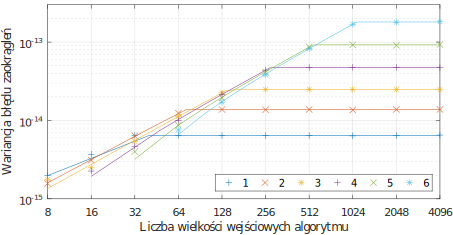
\includegraphics{obrazki/dwt_rerror_coif5}
\makecaption{fig:dwt_rerror_coif5}{Zależność wariancji błędu zaokrągleń od liczby iteracji procesu dekompozycji sygnału oraz liczby wielkości wejściowych dla falki \enquote{coif5} i długości słowa~\qty{32}{\bitOw}}
\end{center}
\end{figure}

\begin{table}[htb!]
\begin{center}
\makecaption{tab:varnum_db2_2_f16}{Wariancja błędu zaokrągleń kolejnych wielkości wyjściowych algorytmu dyskretnej transformacji falkowej dla falki \enquote{db2} przy dwóch iteracjach procesu dekompozycji, dla liczb o długości~\qty{16}{\bitOw}, w zależności od zakresu wielkości wejściowych}
\begin{tabular}[c]{| c *{6}{|S[table-format = 1.2e+1, mode = math]} |} \hline
\multirow{2}{*}{$X$} & \multicolumn{6}{ c |}{\textbf{Zakres wielkości wejściowych algorytmu}} \\ \cline{2-7}
& \text{$<-1;1>$} & \text{$<-2;2>$} & \text{$<-3;3>$} & \text{$<0;2>$} & \text{$<0;4>$} & \text{$<3;9>$} \\ \hline
$S_{2,0}$ & 1.03e-7 & 4.12e-7 & 9.74e-7 & 7.08e-7 & 2.83e-6 & 2.16e-5 \\ \hline
$S_{2,1}$ & 1.11e-7 & 4.43e-7 & 1.01e-6 & 9.55e-7 & 3.82e-6 & 2.75e-5 \\ \hline
$T_{2,0}$ & 1.31e-7 & 5.24e-7 & 1.21e-6 & 2.87e-7 & 1.15e-6 & 7.06e-6 \\ \hline
$T_{2,1}$ & 1.07e-7 & 4.29e-7 & 9.73e-7 & 3.36e-7 & 1.34e-6 & 9.30e-6 \\ \hline
$T_{1,0}$ & 7.09e-8 & 2.85e-7 & 6.99e-7 & 1.65e-7 & 3.56e-7 & 4.29e-6 \\ \hline
$T_{1,1}$ & 5.83e-8 & 2.33e-7 & 5.87e-7 & 1.49e-7 & 5.95e-7 & 4.05e-6 \\ \hline
$T_{1,2}$ & 5.84e-8 & 2.34e-7 & 5.85e-7 & 1.49e-7 & 5.97e-7 & 4.05e-6 \\ \hline
$T_{1,3}$ & 5.53e-8 & 2.21e-7 & 5.41e-7 & 1.78e-7 & 7.08e-7 & 5.26e-6 \\ \hline
\end{tabular}
\end{center}
\end{table}

\begin{table}[htb!]
\begin{center}
\makecaption{tab:varnum_db2_2_f32}{Wariancja błędu zaokrągleń kolejnych wielkości wyjściowych algorytmu dyskretnej transformacji falkowej dla falki \enquote{db2} przy dwóch iteracjach procesu dekompozycji, dla liczb o długości~\qty{32}{\bitOw}, w zależności od zakresu wielkości wejściowych}
\begin{tabular}[c]{| c *{6}{|S[table-format = 1.2e+2, mode = math]} |} \hline
\multirow{2}{*}{$X$} & \multicolumn{6}{ c |}{\textbf{Zakres wielkości wejściowych algorytmu}} \\ \cline{2-7}
& \text{$<-1;1>$} & \text{$<-2;2>$} & \text{$<-3;3>$} & \text{$<0;2>$} & \text{$<0;4>$} & \text{$<3;9>$} \\ \hline
$S_{2,0}$ & 1.40e-15 & 5.57e-15 & 1.30e-14 & 9.29e-15 & 3.71e-14 & 2.78e-13 \\ \hline
$S_{2,1}$ & 1.40e-15 & 5.61e-15 & 1.29e-14 & 1.25e-14 & 5.00e-14 & 3.54e-13 \\ \hline
$T_{2,0}$ & 1.71e-15 & 6.83e-15 & 1.58e-14 & 3.33e-15 & 1.33e-14 & 7.78e-14 \\ \hline
$T_{2,1}$ & 1.39e-15 & 5.56e-15 & 1.29e-14 & 4.27e-15 & 1.71e-14 & 1.16e-13 \\ \hline
$T_{1,0}$ & 8.28e-16 & 3.54e-15 & 8.38e-15 & 1.70e-15 & 6.84e-15 & 4.25e-14 \\ \hline
$T_{1,1}$ & 6.82e-16 & 2.72e-15 & 6.67e-15 & 1.46e-15 & 5.84e-15 & 4.02e-14 \\ \hline
$T_{1,2}$ & 6.82e-16 & 2.72e-15 & 6.66e-15 & 1.47e-15 & 5.86e-15 & 4.02e-14 \\ \hline
$T_{1,3}$ & 6.68e-16 & 2.67e-15 & 6.48e-15 & 2.02e-15 & 8.10e-15 & 6.15e-14 \\ \hline
\end{tabular}
\end{center}
\end{table}

\begin{table}[htb!]
\begin{center}
\makecaption{tab:varnum_db2_5_f16}{Wariancja błędu zaokrągleń kolejnych grup wielkości wyjściowych algorytmu dyskretnej transformacji falkowej dla falki \enquote{db2} przy pięciu iteracjach procesu dekompozycji, dla liczb o długości~\qty{16}{\bitOw}, w zależności od liczby wielkości wejściowych}
\begin{tabular}[c]{| c *{6}{|S[table-format = 1.2e+1, mode = math]} |} \hline
\multirow{2}{*}{$N$} & \multicolumn{6}{ c |}{\textbf{Skala wielkości wyjściowych algorytmu}} \\ \cline{2-7}
& \text{$S_5$} & \text{$T_5$} & \text{$T_4$} & \text{$T_3$} & \text{$T_2$} & \text{$T_1$} \\ \hline
\textbf{64}   & 4.91e-7 & 5.31e-7 & 3.94e-7 & 2.09e-7 & 1.23e-7 & 5.86e-8 \\ \hline
\textbf{128}  & 7.51e-7 & 7.08e-7 & 3.87e-7 & 2.07e-7 & 1.22e-7 & 5.85e-8 \\ \hline
\textbf{256}  & 8.59e-7 & 6.99e-7 & 3.85e-7 & 2.05e-7 & 1.21e-7 & 5.84e-8 \\ \hline
\textbf{512}  & 9.19e-7 & 6.89e-7 & 3.81e-7 & 2.04e-7 & 1.21e-7 & 5.84e-8 \\ \hline
\textbf{1024} & 9.47e-7 & 6.85e-7 & 3.80e-7 & 2.04e-7 & 1.21e-7 & 5.84e-8 \\ \hline
\textbf{2048} & 9.58e-7 & 6.84e-7 & 3.80e-7 & 2.04e-7 & 1.21e-7 & 5.84e-8 \\ \hline
\textbf{4096} & 9.66e-7 & 6.83e-7 & 3.80e-7 & 2.04e-7 & 1.21e-7 & 5.84e-8 \\ \hline
\end{tabular}
\end{center}
\end{table}

\begin{table}[htb!]
\begin{center}
\makecaption{tab:varnum_db2_5_f32}{Wariancja błędu zaokrągleń kolejnych grup wielkości wyjściowych algorytmu dyskretnej transformacji falkowej dla falki \enquote{db2} przy pięciu iteracjach procesu dekompozycji, dla liczb o długości~\qty{32}{\bitOw}, w zależności od liczby wielkości wejściowych}
\begin{tabular}[c]{| c *{6}{|S[table-format = 1.2e+2, mode = math]} |} \hline
\multirow{2}{*}{$N$} & \multicolumn{6}{ c |}{\textbf{Skala wielkości wyjściowych algorytmu}} \\ \cline{2-7}
& \text{$S_5$} & \text{$T_5$} & \text{$T_4$} & \text{$T_3$} & \text{$T_2$} & \text{$T_1$} \\ \hline
\textbf{64}   & 6.83e-15 & 7.93e-15 & 5.42e-15 & 2.86e-15 & 1.62e-15 & 7.12e-16 \\ \hline
\textbf{128}  & 1.15e-14 & 1.02e-14 & 5.39e-15 & 2.79e-15 & 1.58e-15 & 6.98e-16 \\ \hline
\textbf{256}  & 1.34e-14 & 1.03e-14 & 5.30e-15 & 2.76e-15 & 1.56e-15 & 6.90e-16 \\ \hline
\textbf{512}  & 1.44e-14 & 1.03e-14 & 5.25e-15 & 2.73e-15 & 1.55e-15 & 6.85e-16 \\ \hline
\textbf{1024} & 1.49e-14 & 1.03e-14 & 5.23e-15 & 2.72e-15 & 1.55e-15 & 6.84e-16 \\ \hline
\textbf{2048} & 1.51e-14 & 1.03e-14 & 5.22e-15 & 2.72e-15 & 1.55e-15 & 6.84e-16 \\ \hline
\textbf{4096} & 1.52e-14 & 1.03e-14 & 5.22e-15 & 2.72e-15 & 1.55e-15 & 6.84e-16 \\ \hline
\end{tabular}
\end{center}
\end{table}

Na podstawie rysunku~\ref{fig:dwt_rerror_coif5} zauważyć można liniowy wzrost wariancji sygnału błędu zaokrągleń w funkcji liczby wielkości wejściowych, przy czym wzrost ten ustaje, gdy przestaje zwiększać się liczba operacji arytmetycznych, tj. dla takiej liczby wielkości wejściowych, która jest równa liczbie niezerowych współczynników skalujących dla analizowanego poziomu dekompozycji sygnału. W przypadku tej samej liczby wielkości wejściowych wariancja błędu rośnie wraz ze wzrostem liczby iteracji procesu dekompozycji sygnału, ponieważ zwiększa się liczba niezerowych współczynników skalujących. Można zatem stwierdzić, że wariancja błędu zaokrągleń związana jest w bezpośrednio z liczbą przeprowadzanych operacji arytmetycznych, zatem zależy od liczby współczynników skalujących oraz liczby wielkości wejściowych algorytmu.

\begin{table}[htb!]
\begin{center}
\makecaption{tab:varnum_spline4_4_5_f16}{Wariancja błędu zaokrągleń kolejnych grup wielkości wyjściowych algorytmu dyskretnej transformacji falkowej dla falki \enquote{spline2:4} przy pięciu iteracjach procesu dekompozycji, dla liczb o długości~\qty{16}{\bitOw}, w zależności od liczby wielkości wejściowych}
\begin{tabular}[c]{| c *{6}{|S[table-format = 1.2e+1, mode = math]} |} \hline
\multirow{2}{*}{$N$} & \multicolumn{6}{ c |}{\textbf{Skala wielkości wyjściowych algorytmu}} \\ \cline{2-7}
& \text{$S_5$} & \text{$T_5$} & \text{$T_4$} & \text{$T_3$} & \text{$T_2$} & \text{$T_1$} \\ \hline
\textbf{64}   & 1.07e-6 & 1.02e-6 & 8.94e-7 & 5.05e-7 & 1.83e-7 & 4.76e-8 \\ \hline
\textbf{128}  & 1.75e-6 & 1.59e-6 & 9.22e-7 & 4.96e-7 & 1.80e-7 & 4.64e-8 \\ \hline
\textbf{256}  & 2.61e-6 & 1.67e-6 & 9.11e-7 & 4.91e-7 & 1.77e-7 & 4.58e-8 \\ \hline
\textbf{512}  & 2.60e-6 & 1.69e-6 & 9.05e-7 & 4.89e-7 & 1.76e-7 & 4.55e-8 \\ \hline
\textbf{1024} & 2.58e-6 & 1.71e-6 & 9.02e-7 & 4.88e-7 & 1.75e-7 & 4.53e-8 \\ \hline
\textbf{2048} & 2.58e-6 & 1.71e-6 & 9.00e-7 & 4.87e-7 & 1.75e-7 & 4.53e-8 \\ \hline
\textbf{4096} & 2.58e-6 & 1.72e-6 & 9.00e-7 & 4.87e-7 & 1.75e-7 & 4.53e-8 \\ \hline
\end{tabular}
\end{center}
\end{table}

\begin{table}[htb!]
\begin{center}
\makecaption{tab:varnum_spline4_4_5_f32}{Wariancja błędu zaokrągleń kolejnych grup wielkości wyjściowych algorytmu dyskretnej transformacji falkowej dla falki \enquote{spline2:4} przy pięciu iteracjach procesu dekompozycji, dla liczb o długości~\qty{32}{\bitOw}, w zależności od liczby wielkości wejściowych}
\begin{tabular}[c]{| c *{6}{|S[table-format = 1.2e+2, mode = math]} |} \hline
\multirow{2}{*}{$N$} & \multicolumn{6}{ c |}{\textbf{Skala wielkości wyjściowych algorytmu}} \\ \cline{2-7}
& \text{$S_5$} & \text{$T_5$} & \text{$T_4$} & \text{$T_3$} & \text{$T_2$} & \text{$T_1$} \\ \hline
\textbf{64}   & 1.51e-14 & 1.44e-14 & 1.26e-14 & 6.54e-15 & 2.33e-15 & 5.44e-16 \\ \hline
\textbf{128}  & 2.52e-14 & 2.37e-14 & 1.45e-14 & 6.50e-15 & 2.27e-15 & 5.29e-16 \\ \hline
\textbf{256}  & 4.72e-14 & 2.91e-14 & 1.45e-14 & 6.40e-15 & 2.24e-15 & 5.22e-16 \\ \hline
\textbf{512}  & 4.72e-14 & 2.98e-14 & 1.44e-14 & 6.36e-15 & 2.23e-15 & 5.17e-16 \\ \hline
\textbf{1024} & 4.71e-14 & 3.01e-14 & 1.43e-14 & 6.35e-15 & 2.22e-15 & 5.16e-16 \\ \hline
\textbf{2048} & 4.72e-14 & 3.03e-14 & 1.43e-14 & 6.35e-15 & 2.22e-15 & 5.16e-16 \\ \hline
\textbf{4096} & 4.72e-14 & 3.04e-14 & 1.43e-14 & 6.35e-15 & 2.22e-15 & 5.16e-16 \\ \hline
\end{tabular}
\end{center}
\end{table}

Analizując przedstawione na rysunku~\ref{fig:dwt_rhist_coif5} histogramy zauważyć można, że kształt rozkładu sygnału błędów własnych jest zbliżony do kształtu rozkładu normalnego, natomiast dla poziomu ufności $\alpha = \qty{95}{\percent}$ współczynnik kształtu wynosi około~\num{2.16}. Wobec powyższych, aby możliwe było oszacowanie wartości współczynników koherencji zgodnie z równaniem~\eqref{eq:unc_coher}, konieczne jest wyznaczenie wartości współczynników kształtu, analogicznie jak miało to miejsce w poprzednim rozdziale. Zgodnie z równaniem~\eqref{eq:unc_shapertwo}, stosując metodę Monte-Carlo, oszacowano wartości współczynników kształtu dla sygnału błędu własnego oraz sygnałów błędów o typowych kształtach funkcji gęstości prawdopodobieństwa, a uzyskane wyniki zestawiono w tabeli~\ref{tab:unc_shapedwt}. Z uwagi na fakt, że uzyskane rozkłady sygnałów błędów własnych cechowały się bardzo zbliżonym kształtem, przedstawione wyniki stanowią uśrednione wartości dla wszystkich przeprowadzonych wcześniej eksperymentów.

Stosowanie liczb rzeczywistych o długości słowa~\qty{16}{bitów} pozwala zmniejszyć czas obliczeń oraz rozmiar wymaganej pamięci operacyjnej w stosunku do analogicznego przypadku wykorzystującego liczby o długości słowa~\qty{32}{\bitOw}~\cite{reay_dsp, gcc_manual}. Wariant ten wprowadza jednak znacznie większe błędy związane z zaokrągleniami ze względu na ograniczoną precyzję stosowanego zapisu liczb. Należy zatem tak dobrać długość słowa, aby wariancja sygnału błędu zaokrągleń była możliwie mała w stosunku do wariancji pozostałych sygnałów błędów obecnych w przetwarzanym sygnale, przez co w efekcie sygnał błędu własnego nie wpływał znacząco na wypadkowy sygnał błędu.

Jako, że zakres wielkości wejściowych algorytmu transformacji falkowej również wpływa na wprowadzane błędy zaokrągleń, należy brać ten czynnik pod uwagę podczas analizy projektowanego toru pomiarowego. Należy zatem tak dobrać warunki eksperymentu mającego na celu identyfikacje parametrów sygnału błędu zaokrągleń, aby w jak największym stopniu były one zbieżne z warunkami rzeczywistymi. Analizując przedstawione wyniki zauważyć można, że wraz ze wzrostem zakresu wielkości wejściowych wariancja błędu zaokrągleń wzrasta. Zależność ta wynika bezpośrednio z właściwości stosowanej metody zapisu liczb zmiennoprzecinkowych i została szerzej opisana w publikacji~\cite{benz_floats}.

\begin{table}[htb!]
\begin{center}
\makecaption{tab:unc_shapedwt}{Wartości współczynników kształtu dla typowych kształtów rozkładów oraz rozkładu błędu zaokrągleń algorytmu transformacji falkowej, gdzie kolejne symbole oznaczają rozkład: (n)~normalny, (u)~jednostajny, (t)~trójkątny, (d)~dwumodalny, (r)~zaokrągleń}
\begin{tabular}[c]{| c *{5}{| S[table-format = +1.3] } |} \hline
$s_{r,*}$ & \textbf{$n$} & \textbf{$u$} & \textbf{$t$} & \textbf{$d$} & \textbf{$r$} \\ \hline
$r$       & -0.009       & 0.066        & -0.010       & 0.197        & 0.027        \\ \hline
\end{tabular}
\end{center}
\end{table}

\begin{figure}[htb!]
\begin{center}
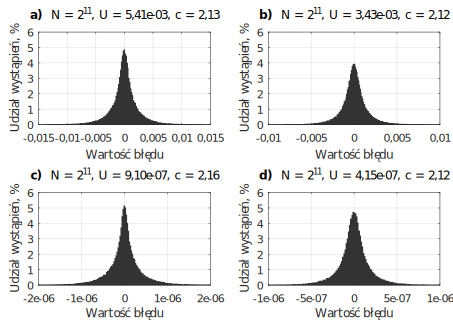
\includegraphics{obrazki/hist_numerr_coif5}
\makecaption{fig:dwt_rhist_coif5}{Histogramy błędu własnego zaokrągleń dla falki \enquote{coif5} przy sześciu iteracjach procesu dekompozycji, dla $N$ wielkości wejściowych, przy długości słowa równej \textbf{a)}, \textbf{b)}~\qty{16}{\bitOw}, \textbf{c)}, \textbf{d)}~\qty{32}{\bitOw}}
\end{center}
\end{figure}

Ze względu na fakt, że przeprowadzone eksperymenty wykazały zbliżone kształty rozkładu realizacji sygnału błędu zaokrągleń niezależnie od parametrów analizowanego algorytmu, w dalszej cześć pracy przyjmuje się, że współczynnik kształtu oznaczony symbolem $c_{z} = \num{2.16}$ odpowiadać będzie sygnałowi błędu zaokrągleń.

\section{Implementacja okna pomiarowego}

Identycznie, jak w przypadku innych algorytmów przetwarzających ciągi wielkości wejściowych, dla algorytmu transformacji falkowej stosować można wybrane okno pomiarowe. Wprowadzenie okna pomiarowego oznaczonego jako $w(n)$ można przedstawić za pomocą modyfikacji równania~\eqref{eq:alg_out_single} jako:
\begin{equation}
X \emb{i} = a_{i, 0} w \emb{0} x \emb{0} + a_{i, 1} w \emb{1} x \emb{1} + \hdots + a_{i, N-1} w \emb{N-1} x \emb{N-1} \label{eq:wt_singlewindow}.
\end{equation}
Na podstawie przedstawionego równania zauważyć można, że wprowadzenie okna pomiarowego opisać można również za pomocą modyfikacji współczynników macierzy transformacji algorytmu zgodnie z zależnością:
\begin{equation}
a'_{i,j} = w \emb{j} a_{i,j} \label{eq:wt_windowmod},
\end{equation}
gdzie $a'_{i,j}$ stanowi nową wartość współczynnika macierzy transformacji algorytmu. Użyta funkcja $w(n)$ powinna być opisana dla wartości $n$ w przedziale $<0;N-1>$. Należy zaznaczyć, że stosowanie okna pomiarowego będzie miało wpływ na widmo sygnałów związanych z kolejnymi wielkościami wyjściowymi algorytmu.

Wybrane okna pomiarowe opisane w literaturze~\cite{oppenheim_dsp, oppenheim_sns, proakis_dsp} to okna: trójkątne~\eqref{eq:wnd_triang}, sinusoidalne~\eqref{eq:wnd_sine}, Gaussa~\eqref{eq:wnd_gauss}, Hamminga~\eqref{eq:wnd_hamming}, Hanna~\eqref{eq:wnd_hann} oraz Welcha~\eqref{eq:wnd_welch}, które opisać można następującymi równaniami:
\begin{gather}
w_{tr} \emb{n} = 1 - \left| \frac{n - \frac{N-1}{2}}{\frac{N}{2}} \right| \label{eq:wnd_triang}, \\
w_{sn} \emb{n} = \sin \left( \frac{\pi n}{N} \right) \label{eq:wnd_sine}, \\
w_{ga} \emb{n} = \exp \left(-\frac{1}{2} \left( \frac{n - \frac{N-1}{2}}{\sigma \frac{\emb{N-1}}{2}} \right)^{2} \right) \label{eq:wnd_gauss}, \\
w_{hm} \emb{n} = \num{0.5384} - \num{0.4616} \cos \left( \frac{2 \pi n}{N} \right) \label{eq:wnd_hamming}, \\
w_{hn} \emb{n} = \num{0.5} \left(1 - \cos \left( \frac{2 \pi n}{N} \right) \right) \label{eq:wnd_hann}, \\
w_{wh} \emb{n} = 1 - \left( \frac{n - \frac{N}{2}}{\frac{N}{2}} \right)^{2} \label{eq:wnd_welch}.
\end{gather}
W dalszej części pracy stosuje się okno prostokątne, w którym $w(n) = 1$, o ile nie został zaznaczony fakt stosowania innego okna pomiarowego.

Implementacja okna pomiarowego, z punktu widzenia przedstawionych w pracy założeń, mogłaby również zostać opisana jako zastosowanie dodatkowego algorytmu. Algorytm ten przetwarzałby $N$ wielkości wejściowych na $M$ wielkości wyjściowych, gdzie $N = M$. Macierz transformacji omawianego algorytmu byłaby macierzą diagonalną, przy czym wartości kolejnych współczynników odpowiadałyby wyznaczonym wagom dla $i$-tej wielkości okna. Z praktycznego punktu widzenia zaproponowana metoda modyfikacji wartości współczynników transformacji algorytmu transformacji falkowej wydaje się jednak bardziej korzystna. Na tej samej zasadzie istnieje możliwość implementacji innych modyfikacji, np. wprowadzenia dodatkowego filtru. Jako, że algorytm dyskretnej transformacji sam w sobie implementuje dla kolejnych wielkości wyjściowych podział tych wielkości na odpowiadające im okna pomiarowe, stosowanie dodatkowego okna pomiarowego nie jest tak popularne, jak w przypadku innych algorytmów (np. algorytmu \enquote{DFT}).

Jako, że wprowadzenie okna pomiarowego objawia się zmianą wypadkowej transmitancji związanej z wielkościami wyjściowymi algorytmu, działanie to wpływa na przenoszone z wejścia na wyjście algorytmu sygnały błędów. Aplikację omawianej metody oraz wpływ parametrów okna pomiarowego na przenoszenie błędów losowych przez algorytmy dyskretnej transformacji falkowej opisano w pracy~\cite{auth_window}.

\section{Podsumowanie przedstawionych zależności}

Specyfika algorytmów transformacji falkowej pozwala na analizę właściwości metrologicznych tych algorytmów stosując model błędów opisany w pracy dla cyfrowej cześć toru pomiarowego. W ogólnym przypadku algorytm transformacji falkowej traktować można jako zbiór $K+1$ filtrów, gdzie $K$ jest liczbą iteracji procesu dekompozycji sygnału. Transmitancja kolejnych wielkości wyjściowych związanych z tą samą iteracją procesu dekompozycji sygnału jest identyczna, natomiast na wejście filtru podawane są różne numery próbek wielkości wejściowych poprzedniego etapu dekompozycji, co związane jest z przesunięciem okna pomiarowego. Transmitancja algorytmu może być określona na podstawie znajomości wartości współczynników skalujących, które wykorzystywane są również do wyznaczenia wartości współczynników macierzy transformacji tego algorytmu. Należy zaznaczyć, że w pewnych przypadkach transmitancja każdej wielkości wyjściowej algorytmu może być inna (np. jeżeli stosowane jest okno pomiarowe).
